\documentclass[notitlepage]{revtex4-1}
\usepackage{geometry}
\usepackage{graphicx}
\usepackage{times}
\usepackage{physics}   % for simple physics notation
\usepackage{bm}        % for math
\usepackage{amssymb}   % for math
\usepackage{amsmath}
\usepackage{subfigure}
\usepackage{color}
\usepackage{float}
\usepackage{enumerate}
\usepackage{enumitem}
\usepackage[export]{adjustbox}
\usepackage{comment}
\usepackage{listings}
\usepackage{CJK}
\usepackage{graphicx}
\newcommand{\hilight}[1]{\colorbox{red}{#1}}
%\usepackage{physics}
%\usepackage{enumerate}
%\usepackage{booktabs} % not allowed in Revtex4.1
\begin{document}
\begin{CJK}{UTF8}{bsmi}
\title{First Principle 2017-Fall  Homework 1 Solution}
%\input author_list.tex       % D0 authors (remove the first 3 lines
                             % of this file prior to submission, they
                             % contain a time stamp for the authorlist)
                             % (includes institutions and visitors)
\author{Kai-Hsin Wu (吳愷訢)}
\email{r05222003@ntu.edu.tw}
\affiliation{Department of Physics and Center of Theoretical Sciences, National Taiwan University, Taipei 10607, Taiwan}

\date{\today}
\maketitle

\begin{enumerate}	
	\item The hcp structure is shown as following :
	
		\begin{figure}[!h]
			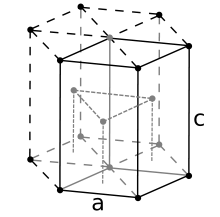
\includegraphics[width=4cm]{{Material/hcp}}
			\caption{hcp structure}
			\label{fig:hcp}
		\end{figure}
		we can calculate the c/a ratio as :
		\begin{equation*}
			\begin{split}
				x &\equiv \frac{c}{2} \\
				x &= \sqrt{ a^2 - (\frac{a}{\sqrt{3}})^2 } = a \cdot \sqrt{\frac{2}{3}} \\
				c/a &= 2 \sqrt{\frac{2}{3}}_{\#}
			\end{split}
		\end{equation*}	

	\item
		\begin{enumerate}[label=(\alph*)] 
			\item 
				\subitem for all $n_i \in$ even with primitive vectors $(2\hat{x} , 2\hat{y} , 2\hat{z})$ , the lattice is a simple cubic lattice with side length 2 origin at $(0\hat{x},0\hat{y},0\hat{z})$
				\subitem for all $n_i \in$ odd with primitive vectors $(2\hat{x} , 2\hat{y} , 2\hat{z})$ , the lattice is also a simple cubic lattice with side length 2 include point $(0\hat{x},0\hat{y},0\hat{z})$ 
			\item 
				\subitem In the case where $\sum_{i} n_i$ is even, this is a simple cubic lattice with side length $\sqrt{3}$ (which can be thought as a $\sqrt{3}$ scaled + $45^o$ rotated version of sc.)
		\end{enumerate}
	\item
		Let's defined the primitive reciprocal lattice is formed by $\langle G_1 , G_2 , G_3 \rangle$.  Which defined as :
		\begin{equation}
			\begin{split}
				G_i \cdot b_j = 2\pi \delta_{ij} 
			\end{split}
		\end{equation} 
		With the known relation:
		\begin{equation}
			\begin{split}
				b_i &\equiv \frac{2\pi (a_j \cross a_k)}{|a_1 \cdot (a_2 \cross a_3) |} \\
				a_i \cdot b_j &= 2\pi \delta_{ij}
			\end{split}
		\end{equation}
		we can see :
		\begin{equation}
			G_i = {a_i}_{\#} 
		\end{equation}			
			
	\item The honeycomb lattice is formed by primitive vectors as the same as parallelogram, with basis contain 2-sites. In which the reciprocal vectors also forms parallelogram. Since the Brillouin zone is just the Wigner-Seitz cell in reciprocal space. The Wigner-Seitz cell formed from parallelogram is hexagonal structure.    
	
	% 5
	\item The first Brilluion zone is the Wigner-Seitz cell in k-space. Which we can represent the boundary point (H,N,P) in terms of reciprocal vector $\vec{b}_i$:
	% ref: http://lampx.tugraz.at/~hadley/ss1/bzones/bcc.php
	\begin{equation}
		\vec{k} = \alpha \vec{b_1} + \beta \vec{b_2} + \gamma \vec{b_3} 
	\end{equation}
	
	For Brilluion zone in bcc lattice, the reciprocal lattice is fcc structure with reciprocal vectors: 
	\begin{align*}
		\vec{b_1} &= \frac{2\pi}{a}(\hat{x} + \hat{z}) \\
		\vec{b_2} &= \frac{2\pi}{a}(\hat{y} + \hat{z}) \\
		\vec{b_3} &= \frac{2\pi}{a}(\hat{y} + \hat{z}) \\
	\end{align*}
	
	The boundary point (H,N,P) thus can be represent in basis of reciprocal vector$\langle\alpha,\beta,\gamma\rangle$:
	\begin{align*}
		H &: \langle -0.5 , 0.5 , 0.5 \rangle \\
		N &: \langle    0 , 0.5 ,   0 \rangle \\
		P &: \langle 0.25 ,0.25 ,0.25 \rangle \\
	\end{align*}
	
	For Brilluion zone in fcc lattice, the reciprocal lattice is bcc structure with reciprocal vectors: 
	% ref: http://lampx.tugraz.at/~hadley/ss1/bzones/fcc.php
	\begin{align*}
	\vec{b_1} &= \frac{2\pi}{a}(\hat{x} -\hat{y} + \hat{z}) \\
	\vec{b_2} &= \frac{2\pi}{a}(\hat{x} + \hat{y} - \hat{z}) \\
	\vec{b_3} &= \frac{2\pi}{a}(-\hat{x} + \hat{y} + \hat{z}) \\
	\end{align*}
	
	The boundary point (X,W,K,U) thus can be represent in basis of reciprocal vector$\langle\alpha,\beta,\gamma\rangle$:
	\begin{align*}
	X &: \langle    0  , 0.5 ,  0.5 \rangle \\
	W &: \langle 0.25  ,0.75 ,  0.5 \rangle \\
	K &: \langle 0.25  ,0.25 , 0.25 \rangle \\
	U &: \langle 0.375 ,0.75 ,0.375 \rangle \\
	\end{align*}
	% 6
	\item 
		\begin{enumerate}[label=(\alph*)]
			\item $GaAs$ 
				\begin{figure}[!h]
					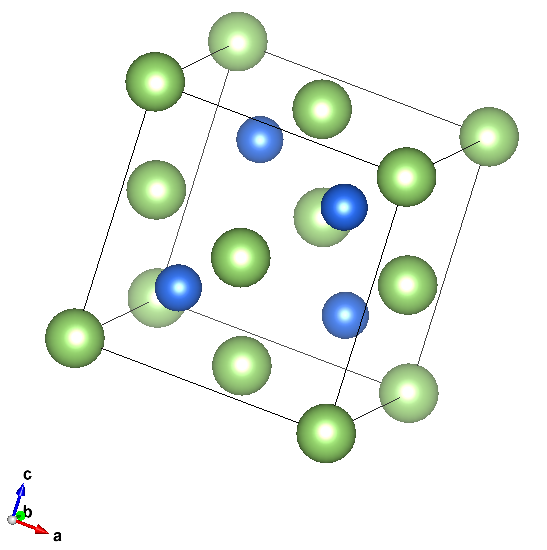
\includegraphics[width=4cm]{{Material/GaAs}}
					\caption{GaAs zinc-blende structure}
					\label{fig:gaas}
				\end{figure}
			
				POSCAR : 
				
\begin{lstlisting}
GaAs
5.653
1.000000000  0.000000000  0.000000000
0.000000000  1.000000000  0.000000000
0.000000000  0.000000000  1.000000000
Ga   As
4    4
Direct
0.000000000  0.000000000  0.000000000
0.000000000  0.500000000  0.500000000
0.500000000  0.500000000  0.000000000
0.500000000  0.000000000  0.500000000
0.750000000  0.250000000  0.750000000
0.250000000  0.250000000  0.250000000
0.250000000  0.750000000  0.750000000
0.750000000  0.750000000  0.250000000
\end{lstlisting}
			\newpage
			\item $NaCl$ 
				\begin{figure}[!h]
					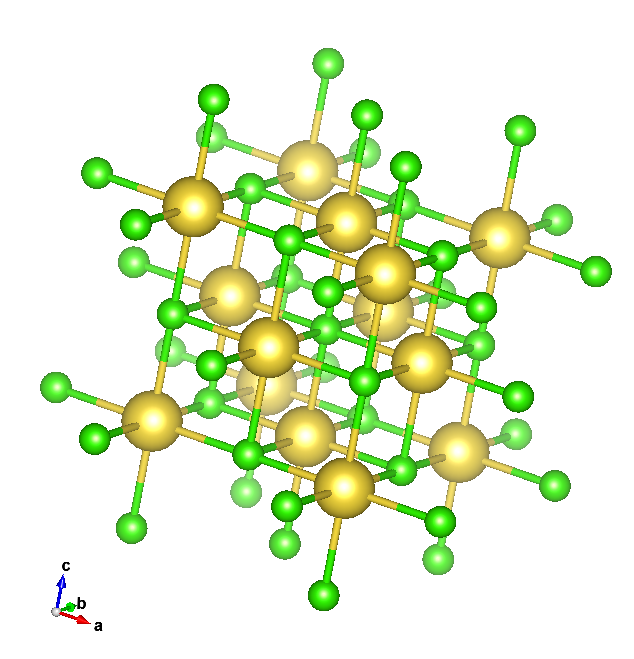
\includegraphics[width=4cm]{{Material/NaCl}}
					\caption{NaCl fcc structure}
					\label{fig:nacl}
				\end{figure}
				
				POSCAR :
\begin{lstlisting}
NaCl
5.64
1.000000000  0.000000000  0.000000000
0.000000000  1.000000000  0.000000000
0.000000000  0.000000000  1.000000000
Na  Cl
4   4
Direct
0.000000000  0.000000000  0.000000000
0.000000000  0.500000000  0.500000000
0.500000000  0.000000000  0.500000000
0.500000000  0.500000000  0.000000000
0.500000000  0.500000000  0.500000000
0.500000000  0.000000000  0.000000000
0.000000000  0.500000000  0.000000000
0.000000000  0.000000000  0.500000000
\end{lstlisting}	
			\newpage
			\item $SrTiO_3$
				\begin{figure}[!h]
					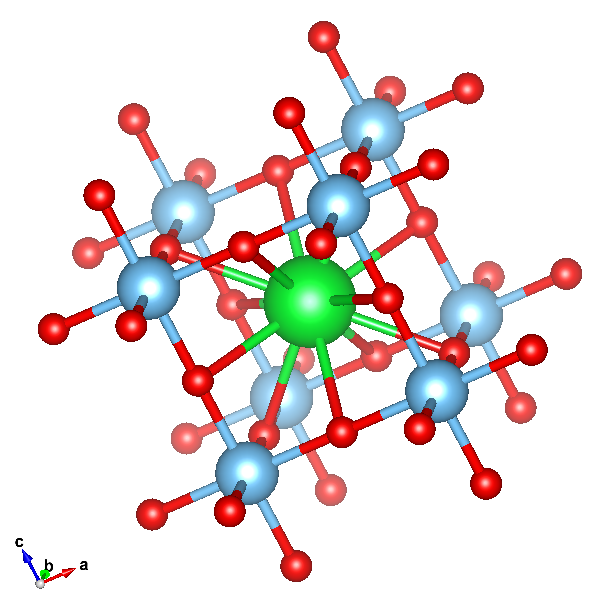
\includegraphics[width=4cm]{{Material/SrTiO3}}
					\caption{SrTiO3 sc structure}
					\label{fig:srtio3}
				\end{figure}
			
			POSCAR :
\begin{lstlisting}
SrTiO3
3.98805
1.000000000  0.000000000  0.000000000
0.000000000  1.000000000  0.000000000
0.000000000  0.000000000  1.000000000
Sr  Ti  O
1   1   3
Direct
0.500000000  0.500000000  0.500000000
0.000000000  0.000000000  0.000000000
0.500000000  0.000000000  0.000000000
0.000000000  0.500000000  0.000000000
0.000000000  0.000000000  0.500000000
\end{lstlisting}	
			\newpage
			\item $2H MoS_2$
				\begin{figure}[!h]
					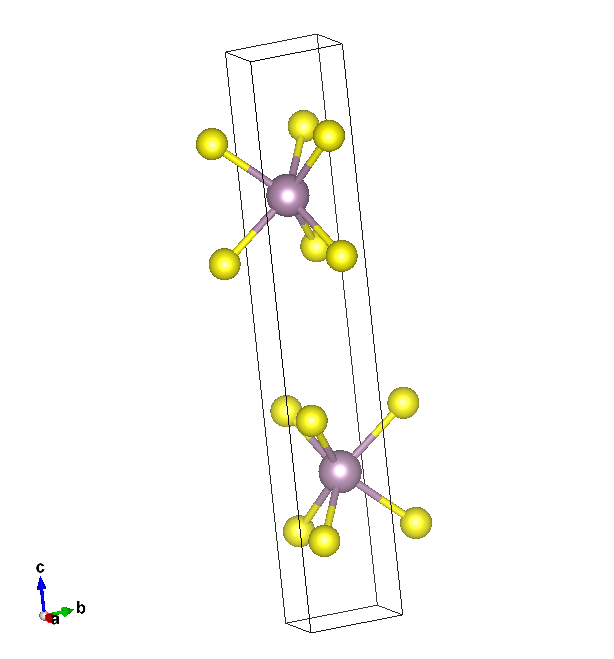
\includegraphics[width=4cm]{{Material/MoS2-2H}}
					\caption{MoS2-2H}
					\label{fig:mos22h}
				\end{figure}
			
			POSCAR :
\begin{lstlisting}
2H-MoS2
3.19
 1.000000000  0.000000000  0.000000000
-0.500000000  0.866025403  0.000000000
 0.000000000  0.000000000  4.664263323
Mo S
2 4
Direct
0.3333333333  0.666666667  0.250000000
0.6666666666  0.333333333  0.750000000
0.3333333333  0.666666667  0.855174000
0.3333333333  0.666666667  0.644826000
0.6666666666  0.333333333  0.355174000
0.6666666666  0.333333333  0.144826000
\end{lstlisting}			
		\end{enumerate}
	
	%7
	\item Considering the general periodic potential with same periodicity of lattice, we can express the potential $U(r)$ as block form :
	\begin{align*}
		U(r) = \sum_{\alpha} U_{\vec{\alpha}} e^{-i\vec{\alpha} \cdot \vec{r}} 
	\end{align*} 
	And block wave function :
	
	\begin{align*}
	\psi_{\vec{k}}(r) &= \sum_{\gamma}C_{\vec{k}-\vec{\gamma}} e^{-i(\vec{k}-\vec{\gamma}) \cdot \vec{r}}
	\end{align*}
	
	where $\vec{\alpha}$ and $\vec{\gamma}$ is reciprocal lattice point. 

	By inserting the block wave function into the Schrödinger equation, we have :
	\begin{align*}
		\left( \frac{\hbar^2}{2m} |\vec{k} - \vec{\gamma}|^2 - 	\epsilon \right) C_{\vec{k} - \vec{\gamma}} + \sum_{\alpha} C_{\vec{k}-\vec{\alpha}} U_{\vec{\alpha}-\vec{\gamma}} = 0 \\
		\left( \epsilon^{0}_{\vec{\gamma}} - 	\epsilon \right) C_{\vec{k} - \vec{\gamma}} + \sum_{\alpha} C_{\vec{k}-\vec{\alpha}} U_{\vec{\alpha}-\vec{\gamma}} = 0
	\end{align*} 
	Where we express the free electron energy at different reciprocal point $\vec{\gamma}$ as $\epsilon^{0}_{\gamma}(\vec{k})$ . 
	
	Thus for the first order approximation with 4 fold degeneracy of free electron energy at $\vec{k}_w$ with given as $\epsilon^{0}_{1}$, $\epsilon^{0}_{2}$, $\epsilon^{0}_{3}$, $\epsilon^{0}_{4}$, we have following equation sets:
	\begin{align*}
		\left( \epsilon - \epsilon^{0}_{1} \right) C_{\vec{k} - \vec{\gamma_{1}}}  &= C_{\vec{k}-\vec{\gamma_{2}}} U_{\vec{\gamma_{2}}-\vec{\gamma_{1}}} 
		                                                                            + C_{\vec{k}-\vec{\gamma_{3}}} U_{\vec{\gamma_{3}}-\vec{\gamma_{1}}} 
		                                                                            + C_{\vec{k}-\vec{\gamma_{4}}} U_{\vec{\gamma_{4}}-\vec{\gamma_{1}}} \\
		\left( \epsilon - \epsilon^{0}_{2} \right) C_{\vec{k} - \vec{\gamma_{2}}}  &= C_{\vec{k}-\vec{\gamma_{1}}} U_{\vec{\gamma_{1}}-\vec{\gamma_{2}}} 
																				    + C_{\vec{k}-\vec{\gamma_{3}}} U_{\vec{\gamma_{3}}-\vec{\gamma_{2}}} 
																				    + C_{\vec{k}-\vec{\gamma_{4}}} U_{\vec{\gamma_{4}}-\vec{\gamma_{2}}} \\
		\left( \epsilon - \epsilon^{0}_{3} \right) C_{\vec{k} - \vec{\gamma_{3}}}  &= C_{\vec{k}-\vec{\gamma_{1}}} U_{\vec{\gamma_{1}}-\vec{\gamma_{3}}} 
																					+ C_{\vec{k}-\vec{\gamma_{2}}} U_{\vec{\gamma_{2}}-\vec{\gamma_{3}}} 
																					+ C_{\vec{k}-\vec{\gamma_{4}}} U_{\vec{\gamma_{4}}-\vec{\gamma_{3}}} \\
		\left( \epsilon - \epsilon^{0}_{4} \right) C_{\vec{k} - \vec{\gamma_{4}}}  &= C_{\vec{k}-\vec{\gamma_{1}}} U_{\vec{\gamma_{1}}-\vec{\gamma_{4}}} 
																					+ C_{\vec{k}-\vec{\gamma_{2}}} U_{\vec{\gamma_{2}}-\vec{\gamma_{4}}} 
																					+ C_{\vec{k}-\vec{\gamma_{3}}} U_{\vec{\gamma_{3}}-\vec{\gamma_{4}}} \\
	\end{align*}  
	
	The above equation can re-align into matrix form :
	\begin{equation}
	\begin{bmatrix}
		\left(  \epsilon^{0}_{1} - \epsilon \right) & U_{\vec{\gamma_{2}}-\vec{\gamma_{1}}}     & U_{\vec{\gamma_{3}}-\vec{\gamma_{1}}}     & U_{\vec{\gamma_{4}}-\vec{\gamma_{1}}} \\
		U_{\vec{\gamma_{1}}-\vec{\gamma_{2}}}     & \left( \epsilon^{0}_{2} -\epsilon  \right) & U_{\vec{\gamma_{3}}-\vec{\gamma_{2}}}     & U_{\vec{\gamma_{4}}-\vec{\gamma_{2}}} \\
		U_{\vec{\gamma_{1}}-\vec{\gamma_{3}}}     & U_{\vec{\gamma_{2}}-\vec{\gamma_{3}}}     & \left( \epsilon^{0}_{3} - \epsilon \right) & U_{\vec{\gamma_{4}}-\vec{\gamma_{3}}} \\
		U_{\vec{\gamma_{1}}-\vec{\gamma_{4}}}     & U_{\vec{\gamma_{2}}-\vec{\gamma_{4}}}     & U_{\vec{\gamma_{3}}-\vec{\gamma_{4}}}    &  \left( \epsilon^{0}_{4} - \epsilon \right) \\
	\end{bmatrix} 
	\begin{bmatrix}
		C_{\vec{k}-\vec{\gamma_{1}}} \\
		C_{\vec{k}-\vec{\gamma_{2}}} \\
		C_{\vec{k}-\vec{\gamma_{3}}} \\
		C_{\vec{k}-\vec{\gamma_{4}}}
	\end{bmatrix} = 0
	\end{equation}
	which the solution is when the determinant = 0. and for fcc :
	
	\begin{figure}[!h]
		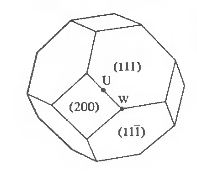
\includegraphics[width=4cm]{{Material/fcc_brilluion}}
		\caption{fcc brilluion zone}
		\label{fig:fccbz}
	\end{figure}
	
	Consider also the symmetry within Brillouin zone, we can easily see :
	
	\begin{align*}
		&U_{\vec{\gamma_{4}-\vec{\gamma_{1}}}} = U_{200} \\
		&U_{\vec{\gamma_{2}-\vec{\gamma_{3}}}} = U_{002} \\
		&U_2 = U_{200} = U_{002} 
	\end{align*}
	\begin{align*}
		&U_{\vec{\gamma_{2}-\vec{\gamma_{1}}}} = U_{111} \\
		&U_{\vec{\gamma_{3}-\vec{\gamma_{1}}}} = U_{11-1} \\
		&U_{\vec{\gamma_{4}-\vec{\gamma_{2}}}} = U_{1-1-1} \\
		&U_1 = U_{111} = U_{11-1} = U_{1-1-1}
	\end{align*}	
	
	thus the solution is:
	\begin{equation}
		\begin{vmatrix}
			( \epsilon^{0}_1 - \epsilon ) & U_1 & U_1 & U_2 \\
			U_1 & ( \epsilon^{0}_2 - \epsilon ) & U_2 & U_1 \\
			U_1 & U_2 &( \epsilon^{0}_3 - \epsilon ) &  U_1 \\
			U_2 & U_1 & U_1 &( \epsilon^{0}_4 - \epsilon )  
		\end{vmatrix} = 0
	\end{equation}
	    
	
	%8 
	\item Considering the block wave function $\psi_{n,\vec{k}}(r)$ with band index $n$, and wave vector$\vec{k}$. The Wannier functions center at lattice position $\vec{R}$ can be written in terms of inverse Fourier transform with constant $\kappa$ :
	\begin{equation}
		\begin{split}
			\phi_n(\vec{r} - \vec{R}) &= \kappa \sum_{\vec{k}} e^{-i \vec{k} \cdot \vec{R}} \psi_{n,\vec{k}}(\vec{r}) 
		\end{split}
	\end{equation}   
	
	Thus :
	\begin{equation}
		\begin{split}
			& \int \phi_n(\vec{r} - \vec{R})\phi_{n'}(\vec{r} - \vec{R}')  d^{D}\vec{r} \\
			&= \kappa^2 \sum_{\vec{k},\vec{h}} e^{i \vec{k} \cdot \vec{R}} e^{-i \vec{h} \cdot \vec{R}'} \int \psi^{*}_{n,\vec{k}}(\vec{r})\psi_{n',\vec{h}}(\vec{r}) d^{D}\vec{r} \\
			&= \kappa^2 \sum_{\vec{k},\vec{h}} e^{i \vec{k} \cdot \vec{R}} e^{-i \vec{h} \cdot \vec{R}'} \delta_{n,n'} \delta_{\vec{k},\vec{h}'} \\
			&= \kappa^2 \delta_{n,n'} \sum_{\vec{k}} e^{i \vec{k} \cdot (\vec{R}-\vec{R}')} \\
			&= \kappa^2 N \delta_{n,n'} \delta_{\vec{R},\vec{R}'} \\
			&\propto \delta_{n,n'} {\delta_{\vec{R},\vec{R}'}}_{\#}
		\end{split}
	\end{equation} 	
	
	The constant $\kappa$ can be derived by the normalization:
	
	\begin{align*}
	 &\int \phi_n(\vec{r} - \vec{R})\phi_{n'}(\vec{r} - \vec{R}') d^{D}\vec{r} = \delta_{n,n'} \delta_{\vec{R},\vec{R}'} \\
	 &\kappa^2 N = 1 \\
	 &\kappa = \frac{1}{\sqrt{N}}_{\#}
	\end{align*}

	%9
	\item The free electron energy is related to the wave vector $\vec{k}$ with a general form :
	\begin{align*}
		E &= \frac{\hbar^2}{2m} |\vec{k}|^2 \\
	\end{align*} 
	For a free end, we can consider a small region with length $L$ in each dimension and impose the periodic boundary condition. 
	\begin{enumerate}[label=(\alph*)]
		\item In case of a channel, where the wave function subject to the constrain $\Psi(x,y,z)=0$ for $|x|>a,|y|>b$,we impose periodic BC in z direction. the possible value of k is constrained as :
		\begin{align*}
			k_x &= \frac{n\pi}{2a} \\
			k_y &= \frac{m\pi}{2b} \\ 
			k_z &= \frac{l2\pi}{Lz} \\
		\end{align*} 
		
		where $n$, $m$ and $l$ are integer. To express the density of state, we see that in $k$ to $k+dk$, $D_v(k)$ is:
		\begin{align*}
			D_v(k)dk &= g\frac{1}{8} 4\pi k^2 / (\frac{\pi^3}{2abL_z}) dk \\
				   &= \frac{gabL_z k^2}{\pi^2} dk 
		\end{align*} 
		where g is the degeneracy. With the relation:
		\begin{align*}
			dk = \frac{\sqrt{m}}{\hbar\sqrt{2}}E^{-1/2} dE  
		\end{align*} 			
		we have the states $D_v(E)$:
		\begin{align*}
			D_v(E)dE &= \frac{\sqrt{2} gabL_z (m)^{3/2}}{\pi^2\hbar^3} E^{1/2} dE \\  
		\end{align*} 		
		Finally divided by the total volumn $4abL_z$, and insert $g=2$ we get DOS (per volumn) :
		\begin{align*}
			D(E)dE  &= \frac{\sqrt{2}m^{3/2}g}{4\pi^2 \hbar^3} E^{1/2} dE \\
			D(E)    &= \frac{(2m)^{3/2}}{2\pi^2 \hbar^3} {E^{1/2}}_{\#}
		\end{align*} 		
				
		\item In case of a slab, where the wave function subject to the constrain $\Psi(x,y,z)=0$ for $|x|>a$,we impose periodic BC in y,z direction. The possible value of k is constrained as :
		\begin{align*}
			k_x &= \frac{n\pi}{2a} \\
			k_y &= \frac{2m\pi}{Ly} \\
			k_z &= \frac{2l\pi}{Lz} \\
		\end{align*} 
		where $n$, $m$, $l$ as integer. To express the density of state, we see that in $k$ to $k+dk$, $D_v(k)$ is:
		\begin{align*}
		D_v(k)dk &= g\frac{1}{8} 4\pi k^2 / (\frac{2\pi^3}{aL_yL_z}) dk \\
				 &= g\frac{ak^2L_yL_z}{4\pi^2} dk
		\end{align*} 
		where g is the degeneracy. With the relation:
		\begin{align*}
		dk = \frac{\sqrt{m}}{\hbar\sqrt{2}}E^{-1/2} dE  
		\end{align*} 			
		we have the states $D_v(E)$:
		\begin{align*}
		D_v(E)dE &= \frac{gaL_zL_y m^{3/2} E^{1/2}}{2\sqrt{2}\hbar^3\pi^2} dE 
		\end{align*} 		
		Finally divided by the total volumn $2aL_yL_z$, and insert $g=2$ we get DOS :
		\begin{align*}
		D(E)dE  &= \frac{m^{3/2}g}{4\sqrt{2}\hbar^3\pi^2} E^{1/2} dE \\
		D(E)    &= \frac{m^{3/2}}{2\sqrt{2}\hbar^3\pi^2} {E^{1/2}}_{\#}
		\end{align*} 		
	\end{enumerate}
	
\end{enumerate}




\bibliographystyle{apsrev4-1}
\bibliography{ref}
	
\end{CJK}
\end{document}

